% g-2 Introduction
\chapter {Introduction}
In particle physics, \gmtwo of the muon, and \gmtwo in general, is an important and deep probe into the Standard Model (SM). The gyromagnetic ratio, $g$, represents the coupling strength of a particle to the type of helicity flipping transitions mediated by magnetic fields, and the $\hbox{--}2$ portion denotes the subtraction of the expected value of the gyromagnetic ratio, leaving only the anomalous magnetic moment, $a$.  The quantity acts as both a seed for new particle physics models and a scythe on proposed models.   Contributions to the quantity depend on the gamut of fundamental interactions and constants of the universe in the SM: quantum electrodynamics (QED), Weak and Strong interactions all playing important roles.  Precision measurement of \gmtwo facilitates development of standard model extensions of somewhat analogous interactions of particles inspired by SM particles.
\todo{expand this a bit, too terse}

\section{History of Experiment}

For many years the value of both $g_e$ and $g_\mu$ were thought to be exactly $2$ as predicted for pure Dirac particles\cite{the-muon-g-2}. And, initial experiments supported the prediction that $g = 2$ \todo{cite initial expt}. That notion, however, had to be reconciled with experiment as measurement precision progressed and statistical tensions arose with the values predicted by theory.  Deviations from a pure Dirac particle were first observed in hyperfine splitting measurements of several different nuclei.  The measured deviations were not statistically significant until Kusch and Foley measured the atomic spectra of several nuclei in 1947 \cite{kusch-foley}.  The theory community quickly resolved the discrepancy with a now standard QED calculation of the lowest order self-interaction for leptons emitting and reabsorbing photons, see figure \ref{fig:schwinger-diagram}.  The Schwinger term, coined after Julian Schwinger, brought experiment and theory back into good agreement.  It served as an early triumph of QED. 

\begin{figure}
\centering
\todo{Add diagram of schwinger term}
\label{fig:schwinger-diagram}
\caption{The Feynman diagram for the so-called Schwinger term.}
\end{figure}

\subsection{Parity Violation}
The first direct measurement of the anomalous magnetic moment, \gmtwo, came later, and the muon \gmtwo much later.  The first measurement of $g_e$ happened in 1953 by H. R. Crane, et al. \todo{can't find pdf of paper}.  Subsequent theoretical calculations and supporting experimental measurements established $g_e$ as the most precisely predicted and measured quantity of QED.  As for measuring $g_\mu$, no one knew how to properly control the polarization of the muons, that is until parity violation of the Weak interaction came to light.  With parity violation baked into the Weak interactions, researchers quickly realized that pion would decay into muons polarized along the beam direction.  

\subsection{CERN-I}
Building off the Weak parity revelation, researchers measured $g_\mu$ for the first time.  In 1960 Columbia personnel measured the quantity to $5\%$, and not long after a more precise measurement came out of CERN and eclipsed it.  The experiment worked by injecting relatively low energy (83 MeV) muons into a long, narrow magnetic trap where the polarized muons would undergo both cyclotron motion and lateral drift. At the opposite end of the magnet, the muons were ejected, tagged for storage time, and stopped where the momentum direction of electron was recorded as recorded as either forward or backward.  Using this technique CERN scientists were able to achieve a precision of $0.4\%$, absolutely phenomenal for the time \cite{cern-i}.  A deviation of $1.6\,\sigma$ was present at the achieved precision.

\begin{figure}
\centering
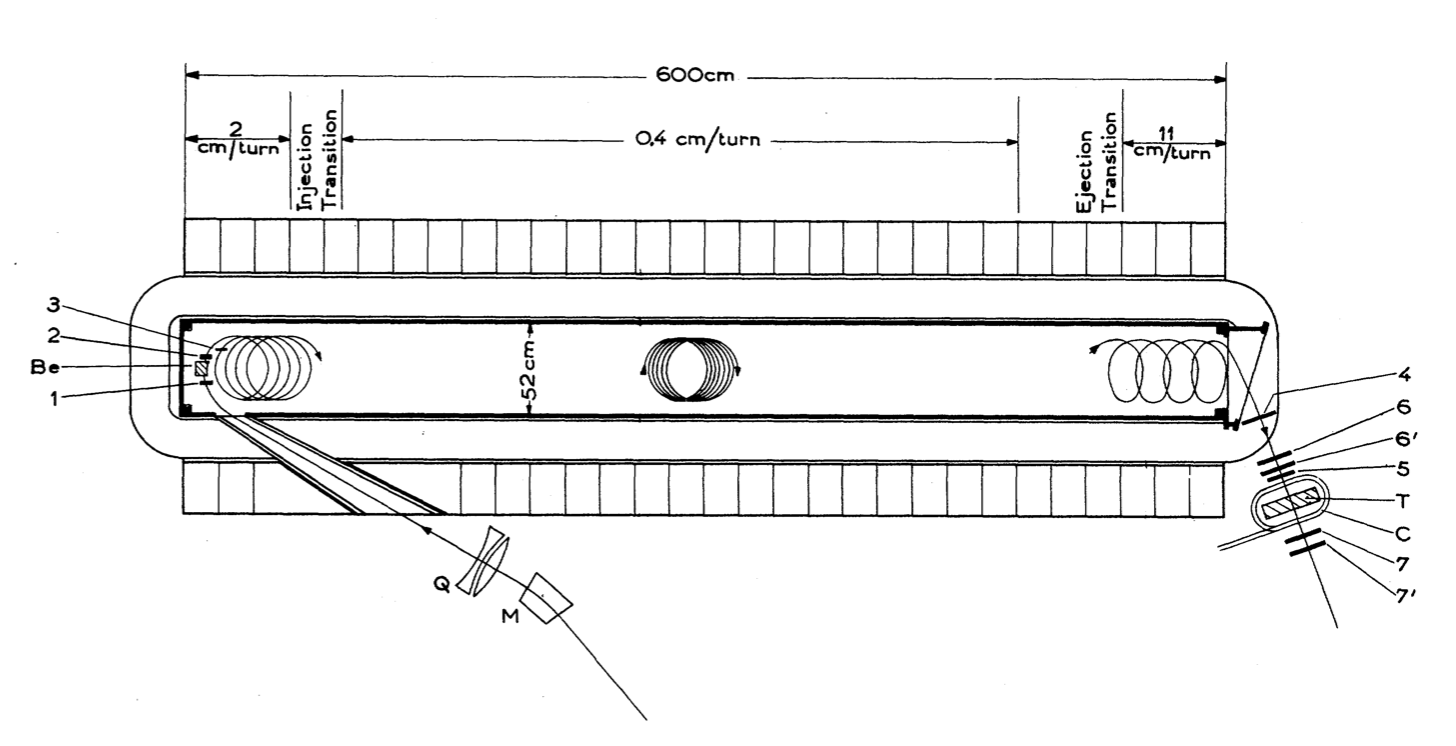
\includegraphics[width=0.9\linewidth]{fig/cern-i-diagram.png}
\label{fig:cern-i-diagram}
\caption{A diagram of the experimental setup in the first muon \gmtwo experiment at CERN. The muons enter from the lower left, go through the energy moderator to put the cyclotron radius at 19cm, drift and circles toward the ejection side of the magnetic, escape from the the magnet, stop in the fiducial block, and decay into an electron with momentum correlated to the spin direction.}
\end{figure}

\subsection{CERN-II}
The second iteration of muon \gmtwo at CERN improved vastly over the first.  CERN-II was the first muon \gmtwo to use the now familiar storage ring \cite{47y-muon-g-2}.  In order to store muons, the experiment injected a beam of protons which hit a pion production target.  A slice of the pion production phase space matched the momentum acceptance of the ring well enough to remain for several revolutions. And, some fraction of the muons produced from pion decay were mostly forward decays that lost a bit of energy and matched the ring's momentum acceptance.  The decay electrons curled inward to electron counting detectors at a rate modulated at \gmtwo frequency.  The injected muons had a relativistic $\gamma$ of 12 which allowed the researchers to measure muon spin precession for more than 130 $\mu s$ which led to determination of $a_\mu$ to \ppm{270}.

\subsection{CERN-III}
The final CERN muon \gmtwo experiment ran from 1969 to 1976.  One major innovation introduced in CERN-III was use of the so-called "magic" momentum. Observe eqn \ref{eqn:full-omega-a}, the equation for spin precession in electromagnetic fields for a relativistic muon.

\begin{equation}
\omega^\prime_a = \omega_a[1 + (1 - 1 / a \beta^2 \gamma^2)(\beta E_r / B)]
\label{eqn:full-omega-a}
\end{equation}

A muon beam at a very specific momentum, \gev{3.094}, cancels the effects of of radial electric fields which allows electrostatic focusing to be used on the muon beam instead of magnetic gradient focusing.  Another major innovation for the third CERN experiment was the use of pion injection instead of proton injection.  The measurement techniques of CERN-III were similar to CERN-II.  With the achieved improvements, the CERN team was able to drive down the uncertainty on $a_\mu$ to \ppm{7}, nearly a 40-fold improvement!

\subsection{E821 at BNL}
The most precise Muon \gmtwo experiment to date, took place at Brookhaven National Laboratory (BNL). The experiment, E821, as it was labeled for high energy physics ledgers pushed precision muon phyiscs to a new level.  E821 needed 400-fold statistics increase over it's predecessor.  In order to accommodate the necessesited higher rates, the decay electron measurement platform was separated into 24 individual calorimeters.  Another critical improvement in the experiment, E821 injected muons rather than pions, or protons.  Muon injection provided a cleaner data earlier in each fill.  The experiment design also focused on improving the homogeneity of the magnetic storage field.  The aperture of the storage region was increased to facilitate a more uniform field across the muon storage volume.  Field measurement was also improved by implementing both a suite of fixed probes always monitoring magnetic field drift outside of the storage region and a trolley outfitted with an array of 17 probes to measure the field in the storage volume periodically.  In the end, the experiment nearly achieved the initial goal of 350 ppb uncertainty on $a_\mu$, actually reaching 540 ppb uncertainty.

The E821 \gmtwo result placed the value at odds with theoretical calculations.  Depending on the theoretical models, the measurement was somewhere around $3.3\sigma - 3.6\sigma$ away from theoretical prediction, a statistical tension.  The tension remained in subsequent years, inspiring a new iteration of the muon \gmtwo experiment at Fermi National Accelerator Laboratory (FNAL). The experiment, E989, reuses the storage ring, superconducting coils, and various components from the BNL experiment.  The goal of E989 is an overall uncertainty of 140 ppb, pushing the tension to a $5\sigma$ discrepancy. Additionally, a sister experiment is being undertaken at J-PARC as a completely independent measurement of muon \gmtwo with similar sensitivity as the BNL experiment.  In a parallel effort, theoretical particle physics researchers have been pushing the precision of calculations to match pace with experiment.

\section{Theory}

\subsection{Magnetic Moment Fundamentals}

A thorough understanding of muon \gmtwo begins with classical model for the magnetic moment of particles. 

\begin{equation}
\vec{\mu} = g \frac{e}{2m}\vec{S}
\label{eqn:spin-magnetic-moment}
\end{equation}


\subsection{Quantum Corrections}

The theoretical contributions to muon \gmtwo come from all corners of particle physics.  The typical diagonalization of the contributions breaks them into QED, Weak, and Strong. The relative sizes of the contributions are displayed in figure \ref{fig:sm-contributions}. The Electro-Weak contributions are well modeled, and theoretical progress involved calculating increasingly intricate Feynman diagrams.  The Strong contributions are trickier and represent a larger challenge to the theory community.  The 

\begin{figure}
\includegraphics[width=0.9\linewidth]{fig/SM-contributions.pdf}
\label{fig:sm-contributions}
\caption{The spectrum of theoretical contributions to muon \gmtwo.}
\end{figure}


\section{Motivation}

\subsection{Statistical Tension}

\subsection{Beyond Standard Model Hints}



